% Lecture Template for ENGR 1120 030 031 E01- Tristan Hill - Spring 2017
% 
% Introduction to MATLAB 
%
% Low Level File IO - 

% Document settings
\documentclass[11pt]{article}
\usepackage[margin=1in]{geometry}
\usepackage[pdftex]{graphicx}
\usepackage{multirow}
\usepackage{setspace}
\usepackage{hyperref}
\usepackage{color,soul}
\usepackage{fancyvrb}
\usepackage{framed}
\usepackage{wasysym}
\usepackage{multicol}

\pagestyle{plain}
\setlength\parindent{0pt}
\hypersetup{
    bookmarks=true,         % show bookmarks bar?
    unicode=false,          % non-Latin characters in Acrobat’s bookmarks
    pdftoolbar=true,        % show Acrobat’s toolbar?
    pdfmenubar=true,        % show Acrobat’s menu?
    pdffitwindow=false,     % window fit to page when opened
    pdfstartview={FitH},    % fits the width of the page to the window
    pdftitle={My title},    % title
    pdfauthor={Author},     % author
    pdfsubject={Subject},   % subject of the document
    pdfcreator={Creator},   % creator of the document
    pdfproducer={Producer}, % producer of the document
    pdfkeywords={keyword1} {key2} {key3}, % list of keywords
    pdfnewwindow=true,      % links in new window
    colorlinks=true,       % false: boxed links; true: colored links
    linkcolor=red,          % color of internal links (change box color with linkbordercolor)
    citecolor=green,        % color of links to bibliography
    filecolor=magenta,      % color of file links
    urlcolor=blue           % color of external links
}

% assignment number 
\newcommand{\NUM}{9 } 
\newcommand{\VSpaceSize}{2mm} 
\newcommand{\HSpaceSize}{2mm} 

\definecolor{mygray}{rgb}{.6, .6, .6}

% [153,50,204] - dark orchid
\definecolor{mypurple}{rgb}{0.6,0.1961,0.8}
%[139,69,19] - saddle brown
\definecolor{mybrown}{rgb}{0.5451,0.2706,0.0745}
\definecolor{mygreen}{rgb}{0,.4,0}


\setulcolor{red} 
\setstcolor{green} 
\sethlcolor{mygray} 

\begin{document}

\textbf{ \LARGE ENGR 1120 Lecture Chapter \NUM - Low-Level File I/O } \\
	
%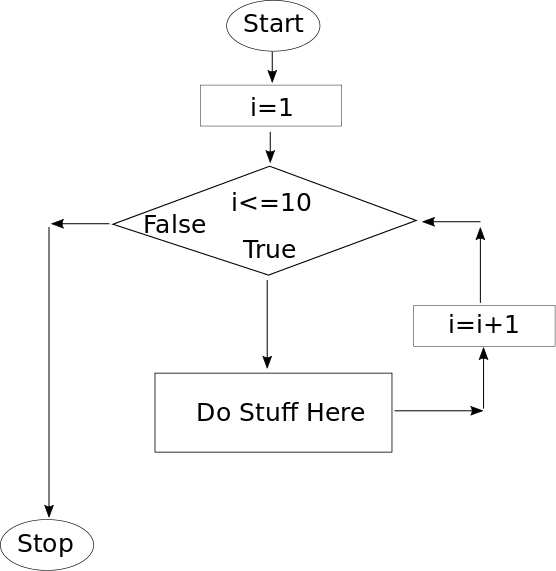
\includegraphics[scale=0.3]{lecture1_fig1.png}\\\\

\Large
\begin{itemize}


	
	\item \textbf{ \LARGE What is a \color{mypurple}Data  File \color{black}? }\\
	
	\begin{itemize}
	\item \textbf{ \LARGE Standard way of organizing data for computer storage. }\\\\\\
	
	\item \textbf{ \LARGE The data can represent many different things but it is all stored \color{mypurple}digitally\color{black}. }\\\\\\
	
	\item \textbf{ \LARGE There are many \color{mypurple}File Types \color{black} used. }\\
	\begin{itemize}
	\item \vspace{10mm}
	\item \vspace{10mm}
	\item \vspace{10mm}
	\end{itemize}
	
	\vspace{10mm}

		\end{itemize}
		\item \textbf{ \LARGE Why do we use \color{mypurple}Data  Files \color{black}? }\\
			\begin{itemize}
	\item \textbf{ \LARGE Organize large amounts of information.}\\\\\\
	
	\item \textbf{ \LARGE Share large amounts of information.}\\\\\\
	

\end{itemize}
		
		
		\item \textbf{ \LARGE  \color{mypurple}File Input \color{black} in MATLAB }\\
		\begin{itemize}
	\item \textbf{ \LARGE get data from a file during \color{mypurple}Program Execution \color{black}  }\\\\
	\item \textbf{ \LARGE data can be stored in a variable(s) to be used by your program  }\\\\
	\end{itemize}
	
	\item \textbf{ \LARGE  MATLAB  \color{mypurple}Syntax\color{black} }\\\\\\
	
	 \scalebox{1.3}{{\fontfamily{qcr}\selectfont \color{black}fid =  fopen(\color{mypurple}'filename.txt' \color{black}, \color{mypurple}'r'\color{black}) }} \\\\\\

 \scalebox{1.3}{{\fontfamily{qcr}\selectfont \color{black}x =  fscanf(\color{black}fid , \color{mypurple}'\%f' \color{black}, 1) }} \\\\\\

 \scalebox{1.3}{{\fontfamily{qcr}\selectfont \color{black}fclose(\color{black}fid) }} \\\\\\
 	
\newpage

	\item \textbf{ \LARGE A few things about the \color{blue}File Identifier \color{black} }\\
\begin{itemize}
	\item \textbf{ \Large  \color{black} the file identifier, fid, gives us information about the {\it fopen}}\vspace{5mm} \\
	
	\item \textbf{ \Large  \color{black}if opened properly the fid will have a positive value}\vspace{5mm} \\
	
	\item \textbf{ \Large  \color{black}if something goes wrong the fid will have a negative value}\vspace{5mm} \\
		\begin{itemize}
			\item File is not in the proper \color{blue} directory \color{black}  \\\\
			\item The \color{mypurple} current folder  \color{black} has not been set properly \\\\
			\item Please organize you file structure! \\\\
		\end{itemize}
	
	\item \textbf{ \Large  \color{black} fid, can also give information about the \color{blue} End Of File\color{black} }\vspace{5mm} \\
	
	 \scalebox{1.3}{{\fontfamily{qcr}\selectfont feof(fid) \color{mygreen} \% returns a boolean }} \\\\\\
 	
 	\item \textbf{ \Large  \color{black} We use this is we do not know how long the file is}\\\\
	
	 \scalebox{1.3}{{\fontfamily{qcr}\selectfont \color{blue}while\color{black}($\sim$feof(fid)) \color{mygreen}  }} \\\\\\
\end{itemize}


		\item \textbf{ \LARGE  \color{mypurple}File Output \color{black} in MATLAB }\\
		\begin{itemize}
	\item \textbf{ \LARGE put data into a file during \color{mypurple}Program Execution \color{black}  }\\\\
	\item \textbf{ \LARGE the file may or may not already exist.  }\\\\
	\end{itemize}
	
	\item \textbf{ \LARGE  MATLAB  \color{mypurple}Syntax\color{black} }\\\\\\
	
	 \scalebox{1.3}{{\fontfamily{qcr}\selectfont \color{black}fid =  fopen(\color{mypurple}'filename.txt' \color{black}, \color{mypurple}'w'\color{black}) }} \\\\\\

 \scalebox{1.3}{{\fontfamily{qcr}\selectfont \color{black}x =  99.9 }} \\\\
 
 \scalebox{1.3}{{\fontfamily{qcr}\selectfont \color{black} fprintf(\color{black}fid , \color{mypurple}'\%f' \color{black}, x) }} \\\\\\

 \scalebox{1.3}{{\fontfamily{qcr}\selectfont \color{black}fclose(\color{black}fid) }} \\\\\\
 	
\newpage
\end{itemize}
	

\end{document}



